\subsection{Adopted programming languages and frameworks}
\hspace{\parindent} The CLup app as already mentioned has been developed in Android Studio, an IDE for building Android apps based on IntelliJ IDEA software from JetBrains. Android Studio can be used with three programming languages - Kotlin, Java, and C++ , all used for object oriented programming of the app. \newline
Our choice was to go with Java since that's the language we're most familiar with and a language that exists a lot longer than Kotlin, which is Google's preferred language for Android app dev, so more examples can be found online for easier referencing. \newline
Java also offers vast and detailed documentation as well as similar syntax to some other more popular languages, contrary to Kotlin. \newline
Android Studio also uses an internal UI design tool, which is based on XML language that uses layouts, items, and resources for designing and creating different app screens. It features a real-time design screen making an UI design a lot smoother and faster experience. \newline
During the development we have used a Google Pixel 3 virtual machine, that is also integrated in Android Studio, for testing and other app-related purposes.\newline 
Several phones of different sizes, vendors, and Android versions have been used for real-life testing, and those are: Samsung Galaxy Note 9, Xiaomi Redmi Note 9 Pro, and Huaweii P Smart.  \newline
Even though our original plan was to use MySQL database for the backend of this project, we have decided to use Google's Firebase that was mentioned as an alternative in the Design document. More details on this design choice in the sections below.

\subsection{Adopted additional algorithms and middleware}
\hspace{\parindent} One of the APIs that was planned to be used, Google Maps API, did not make the cut in this version. The reasoning behind that is already explained in the previous chapter and it touches on the lack of "Book a visit" feature that was not required to be made for smaller groups. Using this API would further complicate things and we did not find it necessary just for the ticket queueing function of the app, since this function would mostly be used on the fly and without too much planning, which would mean that the customers would already know to which store they are going and how to get there. \newline

One of the main challenges of the system was securing a proper encryption for the QR code which is to be scanned by the store manager. If we put no encryption on it, the customers can easily scan the code on their own, see how it looks, and the create their own QR codes to skip lines and get faster access to the store. \newline
For that reason we have decided to use AES or Advanced Encryption Standard which is a specification for electronic data encryption. It is one of the most widely used standards in the world and regarded as one of the most secure. \newline

This standard uses either 128, 192, or 256 bit keys to encode and decode data. It is also symmetrical, making it easier to do encryption/decryption without exchanging keys. \newline

The way AES works is that it takes plaintext and a key, encodes it using a special algorithm, and then sends the ciphertext to the destination. The receiver receiver the ciphertext and decodes it using the same key, getting the original message. \newline

\begin{figure}[H]
\centering
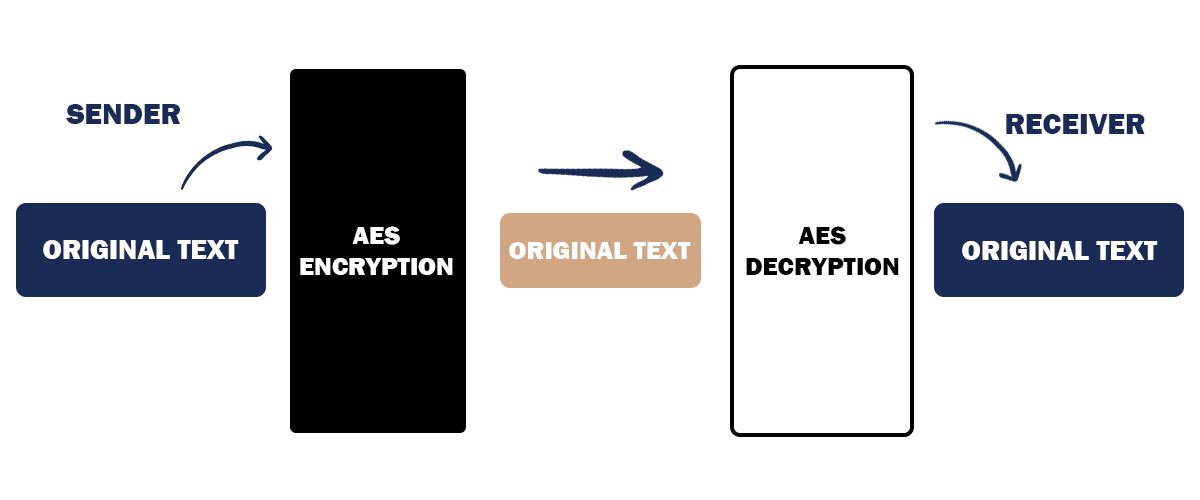
\includegraphics[width=\textwidth]{Images/AES}
\caption{\label{fig:aes}\textbf{AES sketch}}
\end{figure}

Each store in our database has a unique 128 bit key with mixed characters. This key is used for encryption when requesting a ticket and then for decryption when scanning a ticket. The key is not sent at any moment over the network and it's not shown to the customer or the store manager at any time, making the app very secure in that regard.\newline
If user tries to scan the QR code, they will get something like this:\newline

"-112w-22w34w-41w34w-120w2w-22w87w-93w-41w65w11".\newline

Good luck with trying to get any data from that! Even NSA uses it.
Our encryption code generates random signed 8 bit integers which are then interleaved with a letter, "w" in this scenario, for easier decryption later. The code for the algorithm is provided here.\newline

\textbf{Entities - StrongAES}

\begin{lstlisting}
// StrongAES.java
package com.example.clup;

import java.security.Key;
import javax.crypto.Cipher;
import javax.crypto.spec.SecretKeySpec;
public class StrongAES
{
    // function that Encrypts and Decrypts data
    public byte[] AESEncrypt(String plaintext, String key){
        try {
            Key aesKey = new SecretKeySpec(key.getBytes(), "AES");
            Cipher cipher = Cipher.getInstance("AES");
            // encrypt the text
            cipher.init(Cipher.ENCRYPT_MODE, aesKey); // encrypted with a key
            byte[] cy = cipher.doFinal(plaintext.getBytes()); // encryption is returned in bytes[] array
            //System.out.println(cy);
            return cy;
        }
        catch(Exception e){
            //return 'D';
            return "false".getBytes();
        }
    }

    public String AESDecrypt(byte[] cyphertext, String key){
        try {
            Key aesKey = new SecretKeySpec(key.getBytes(), "AES");
            Cipher cipher = Cipher.getInstance("AES");
            cipher.init(Cipher.DECRYPT_MODE, aesKey); // decrypted with a key
            String cy2 = new String(cipher.doFinal(cyphertext)); // decryption is returned in String
            //System.out.println(cy2);
            return cy2;
        }
        catch(Exception e){
            System.err.println(e);
            return "Error";
        }
    }
   }
\end{lstlisting}


\subsection{Database model}
\hspace{\parindent} Google's Firebase is a very powerful databse tool for two reason - it is very simple and it's easily integrated with Android apps. It is not a standard database tool that uses SQL language (it is NoSQL), but rather separates its data by using JSON structures and a classic key-value methodology. Every item can have a key and a value, as well as be a parent and have multiple children. However, any item that has a child or children cannot have any values, but is rather just represented with a key. \newline

This all makes extracting data very simple, but it generates a problem with data multiplication since there is no way of connecting some items with a pointer or by id. What must be done is a manual data copying, which increases size and complexity of the structure. \newline

Android Studio and the whole Android environment has already built in functions that make working with Firebase much easier, which was the main reason for this selection. Functions for user registration and login are already set up and are super secure, not even requiring storing user password in the database. \newline

The whole Firebase interface is also very well done and allows maximum customization as well as adaptability to the certain project. It is located on a Google server, so there is no need to worry about any other sever that runs a normal database, since Google servers are always up and have very small limitations, at least for a smaller scale project. \newline

You can see the way we have structured our database in the following examples. 

\begin{figure}[H]
\centering
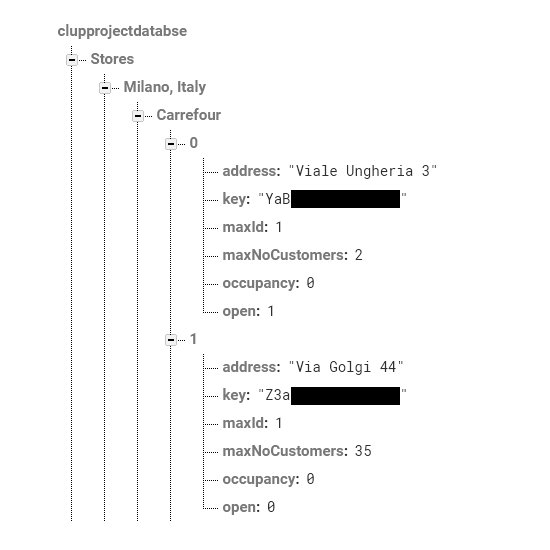
\includegraphics[width=\textwidth]{Images/Firebase1}
\caption{\label{fig:fire1}\textbf{Our Firebase database 1}}
\end{figure}
\begin{figure}[H]
\centering
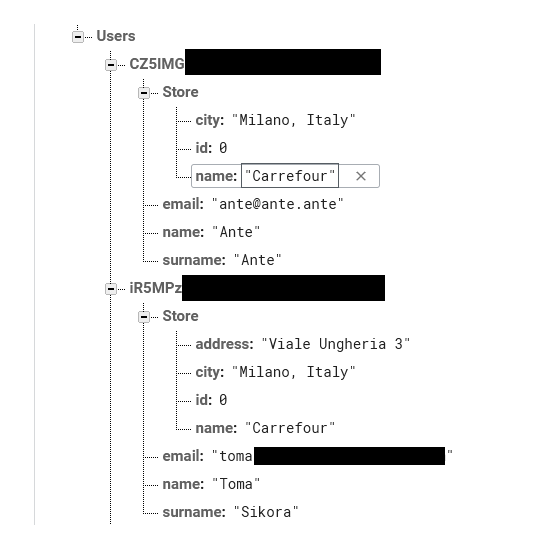
\includegraphics[width=\textwidth]{Images/Firebase2}
\caption{\label{fig:fire2}\textbf{Our Firebase database 2}}
\end{figure}


The two main items are "Stores" and "Users". Stores are ordered by cities, then by store names, and finally by id. Each store has an address, a key, a current ticket id, a maximum number of customers, an occupancy number, and an open indicator. Also, each store has another set of children "Tickets", which is created dynamically. \newline

Each user is defined by "UserID" which is a Firebase identification. Connected to the user are a specific Store, which here only consists of a city, an ID, and a name, so we can reference it in the other "Store" structure, as well as an email, a name, and a surname, with the latter two being used only for registration, which has been omitted from the final app version. Therefore store managers and stores are added manually for additional security and data consistency. \newline

The main Firebase issue is the data retrieval - sometimes the servers take up to 5 seconds to return simple data! In this case it is not a major issue, since the speed is not the most important function of the application, but the server dependability of getting the data back on time can cause some problems. \newline

All in all, in case of a a real-world app for a much larger scale, we would probably transfer to MySQL mainly because of speed and stability which are not strong sides of Firebase. \newline